\chapter{Introduzione e definizione del problema}
\label{chap:introduzione}

L'\textbf{anomaly detection}, o rilevamento delle anomalie, consiste nell'identificare osservazioni che si discostano significativamente dal comportamento prevalente dei dati. Tali deviazioni possono suggerire la presenza di un meccanismo generativo differente e, nei contesti applicativi, segnalare eventi che richiedono un approfondimento \cite{Pang_et_al._2021}.

La difficoltà del problema dipende soprattutto da tre caratteristiche:
\begin{itemize}
    \item \textbf{scarsa conoscenza preliminare}: alcune tipologie di anomalia diventano note soltanto quando si manifestano;
    \item \textbf{eterogeneità}: anomalie diverse possono presentare caratteristiche visive o statistiche molto differenti;
    \item \textbf{rarità}: i campioni anomali sono spesso poco numerosi rispetto a quelli che descrivono il normale funzionamento.
\end{itemize}

Queste caratteristiche rendono difficile raccogliere esempi rappresentativi di tutti i difetti possibili. La ricerca sul rilevamento delle anomalie ha quindi sviluppato metodi capaci di apprendere la regolarità dei dati e di riconoscere deviazioni non necessariamente osservate durante l'addestramento. Tra le principali questioni aperte si distinguono \cite{Pang_et_al._2021}:
\begin{enumerate}
    \item \textbf{Sensibilità e falsi allarmi}. Un basso richiamo (\textit{recall}) indica che una parte delle anomalie non viene rilevata, producendo falsi negativi. Aumentare la sensibilità può però incrementare i falsi positivi, ossia i campioni normali segnalati come anomali. Il compromesso tra questi due errori dipende dall'applicazione.
    \item \textbf{Alta dimensionalità e dipendenze tra osservazioni}. Le deviazioni possono riguardare poche componenti di dati molto complessi. Inoltre, alcune anomalie sono riconoscibili soltanto considerando relazioni spaziali, temporali o contestuali.
    \item \textbf{Disponibilità limitata di dati}. La raccolta e l'annotazione dei difetti possono essere costose. Occorre quindi sfruttare efficacemente i campioni normali e, quando disponibili, le informazioni parzialmente etichettate.
    \item \textbf{Robustezza al rumore}. Etichette errate, disturbi di acquisizione e campioni anomali non riconosciuti possono compromettere l'apprendimento della normalità. La tolleranza a tali contaminazioni deve essere valutata per ciascun metodo.
    \item \textbf{Anomalie complesse}. Oltre alle deviazioni di singole osservazioni, occorre considerare anomalie contestuali, che dipendono dalle condizioni di osservazione, e collettive, che emergono dal comportamento di un gruppo di dati.
    \item \textbf{Interpretabilità}. Nei domini critici è utile comprendere quali informazioni abbiano determinato una segnalazione. La localizzazione di un difetto può supportare l'ispezione umana, ma non costituisce di per sé una spiegazione del comportamento del modello.
\end{enumerate}

Il deep learning consente di apprendere rappresentazioni dei dati senza definire manualmente tutte le caratteristiche rilevanti. Questo può migliorare il rilevamento in scenari complessi; non elimina, tuttavia, i problemi di robustezza, generalizzazione e interpretabilità. Il presente elaborato si concentra sulle anomalie visive nell'ispezione industriale.

\section[Anomalie nella visione artificiale]{Il rilevamento delle anomalie nella visione artificiale}

La \textit{Visual Anomaly Detection} (VAD) identifica, in dati visivi quali immagini o nuvole di punti, elementi che si discostano da una definizione di normalità \cite{Cao_et_al._2024}. Rispetto alla classificazione in cui le classi sono note a priori, il problema richiede di riconoscere anche difetti assenti dai dati di addestramento \cite{Yang_et_al._2021}.

Si distinguono due obiettivi:
\begin{itemize}
    \item \textbf{rilevamento a livello di immagine} (\textit{image-level}): stabilire se un'immagine contenga un'anomalia, mediante un punteggio globale;
    \item \textbf{localizzazione a livello di pixel} (\textit{pixel-level}): assegnare punteggi alle posizioni dell'immagine per individuare le regioni potenzialmente difettose.
\end{itemize}

Una buona discriminazione globale non implica necessariamente una localizzazione accurata. Un modello può segnalare correttamente un'immagine difettosa e produrre, allo stesso tempo, una mappa troppo estesa o incompleta. La distinzione tra i due obiettivi guida la scelta delle metriche e l'interpretazione dei risultati \cite{Yang_et_al._2021,Pang_et_al._2021}.

\subsection{Sfide dei contesti industriali}

L'integrazione di sistemi di visione e sensori nei processi produttivi offre nuove possibilità di controllo automatizzato. Il trasferimento dei metodi dagli scenari di laboratorio alle applicazioni reali richiede però di affrontare lo sbilanciamento dei dati, la variabilità dei difetti e le condizioni di acquisizione \cite{Cui_et_al._2023,Li_et_al._2025}.

\subsubsection{Sbilanciamento delle classi}

Nelle linee di produzione efficienti, i difetti possono essere sporadici. Un classificatore addestrato su dati fortemente sbilanciati rischia di privilegiare la classe normale, trascurando eventi rari ma rilevanti. La scarsità di esempi difettosi motiva l'impiego di approcci che apprendono soprattutto dai campioni conformi \cite{Li_et_al._2025,Aggarwal_et_al._2021}.

\begin{figure}[htbp]
    \centering
    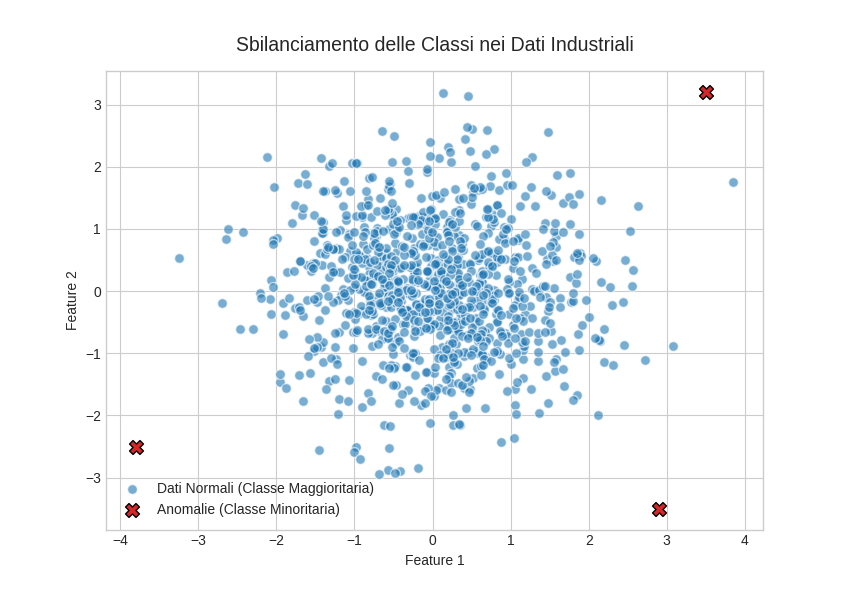
\includegraphics[width=0.8\textwidth]{Sbilaciamento_delle_classi.png}
    \caption{Rappresentazione schematica dello sbilanciamento tra campioni normali ed eventi anomali.}
    \label{fig:sbilanciamento}
\end{figure}

\subsubsection{Variabilità ed eterogeneità delle anomalie}

I difetti possono differire per forma, dimensione, posizione e contrasto rispetto al materiale. Non è quindi realistico assumere di poter rappresentare tutte le loro configurazioni nel training set. Il modello deve distinguere le variazioni compatibili con il prodotto conforme dalle deviazioni significative, generalizzando oltre gli esempi osservati \cite{Aggarwal_et_al._2021,Cui_et_al._2023}.

La Figura~\ref{fig:variabilita_anomalia} illustra, mediante una serie temporale, la distinzione generale tra anomalie puntuali, contestuali e collettive. Nell'ispezione visiva, l'eterogeneità si manifesta invece attraverso alterazioni cromatiche, discontinuità della texture o modifiche della struttura dell'oggetto.

\begin{figure}[htbp]
    \centering
    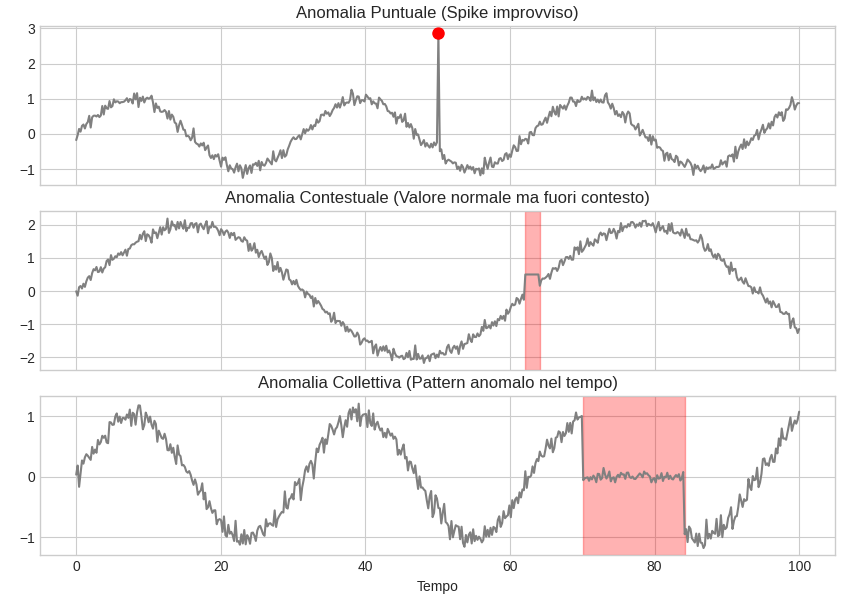
\includegraphics[width=0.8\textwidth]{Variabilita_dell_anomalia.png}
    \caption{Esempio delle tipologie generali di anomalia in una serie temporale: puntuale, contestuale e collettiva.}
    \label{fig:variabilita_anomalia}
\end{figure}

\subsubsection{Dipendenza dal contesto e condizioni di acquisizione}

La normalità dipende dalle condizioni operative. Un valore di temperatura può essere accettabile in una fase produttiva e indicare un guasto in un'altra; analogamente, nell'ispezione visiva, illuminazione, riflessi e variazioni ammesse del materiale possono modificare l'aspetto di un prodotto conforme.

I confini tra variazione normale e difetto possono dunque essere ambigui. Il preprocessing e l'eventuale impiego di informazioni contestuali devono essere progettati in funzione del dominio, per limitare le segnalazioni dovute ai disturbi di acquisizione \cite{Li_et_al._2025,Alzarooni_et_al._2024}. La Figura~\ref{fig:contesto_industriale} esemplifica il ruolo del contesto nella scelta di una soglia di rilevamento.

\begin{figure}[htbp]
    \centering
    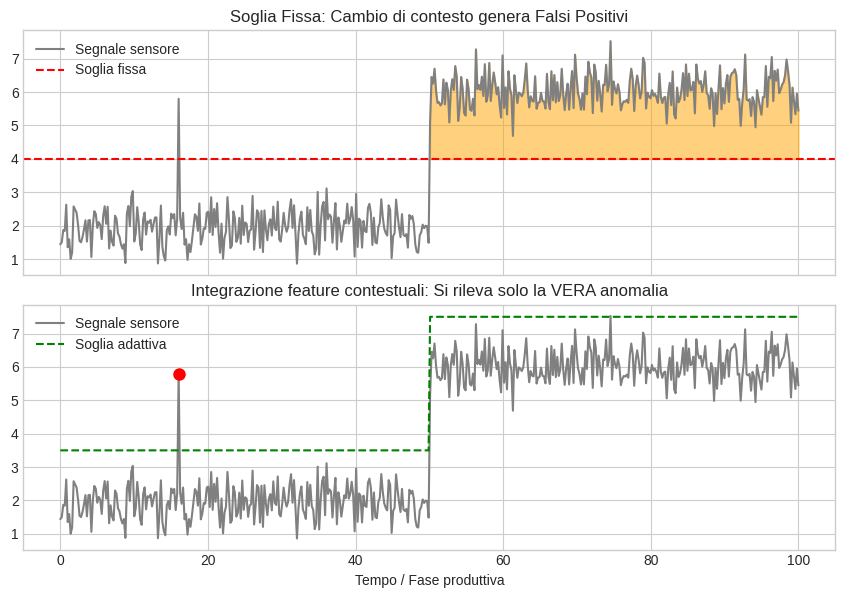
\includegraphics[width=0.8\textwidth]{Soglia_fissa_adattiva.png}
    \caption{Esempio schematico di soglia fissa e soglia adattiva al cambiamento della fase produttiva.}
    \label{fig:contesto_industriale}
\end{figure}

\subsection{Paradigmi di apprendimento e convenzione terminologica}

La disponibilità delle etichette determina quali informazioni possano guidare l'apprendimento. È utile distinguere il paradigma generale dalla granularità delle annotazioni e dalla specifica composizione del training set \cite{Yang_et_al._2021}.

\subsubsection{Apprendimento supervisionato}

Nell'apprendimento supervisionato, ciascun campione è associato a un'etichetta utilizzata durante l'addestramento. Per il rilevamento dei difetti, le etichette possono indicare la conformità dell'intera immagine oppure descrivere le regioni difettose mediante maschere a livello di pixel.

Le annotazioni spaziali richiedono un maggiore lavoro manuale. Le etichette riferite alla sola immagine costituiscono invece una forma di supervisione debole quando l'obiettivo finale è localizzare il difetto. Il vantaggio della supervisione consiste nel fornire esempi espliciti delle anomalie; il limite principale è la necessità di raccogliere campioni sufficientemente rappresentativi \cite{Beitieval_et_al._2024}.

Quando i difetti disponibili sono pochi o poco diversificati, il modello può adattarsi eccessivamente agli esempi osservati e riconoscere con difficoltà anomalie nuove. Questo rischio non implica che tutti i metodi supervisionati falliscano sui difetti sconosciuti, ma rende necessario verificarne la capacità di generalizzazione.

\subsubsection{Apprendimento non supervisionato in senso generale}

Nell'apprendimento non supervisionato non sono disponibili etichette che distinguano i campioni normali da quelli anomali. Molti metodi assumono che le anomalie siano rare e statisticamente distinguibili dalla maggioranza dei dati; il rilevamento dipende quindi dalla rappresentazione adottata e dalla misura di deviazione \cite{Pang_et_al._2021}.

L'assenza di annotazioni riduce il costo di preparazione dei dati, ma non garantisce robustezza alla contaminazione. Se le anomalie influenzano il modello della normalità, possono diventare più difficili da riconoscere. Esistono metodi progettati per affrontare questo problema, la cui efficacia dipende dalle ipotesi e dalle condizioni sperimentali \cite{Lin_et_al._2021}.

\subsubsection{Apprendimento dai soli campioni normali}

Una terza impostazione utilizza un training set composto esclusivamente da campioni noti come normali, senza esempi delle anomalie da rilevare. Nella tassonomia generale dell'anomaly detection, questa impostazione è spesso denominata \textit{semi-supervisionata} \cite{Perez_et_al._2021}. I metodi costruiscono una descrizione della classe normale attraverso confini decisionali, distribuzioni statistiche o rappresentazioni neurali.

Nella letteratura sull'ispezione visiva industriale, lo stesso scenario è comunemente indicato come \textit{unsupervised anomaly detection}, poiché l'apprendimento non richiede esempi annotati dei difetti \cite{Cui_et_al._2023}. Per evitare ambiguità, nel presente elaborato si usa l'espressione \textbf{scenario one-class}: l'adattamento al dominio avviene sui soli campioni normali, mentre le etichette e le maschere del test sono riservate alla valutazione.

Questa convenzione si applica a tutti i modelli selezionati. L'eventuale uso di un backbone pre-addestrato su ImageNet riguarda la provenienza della rappresentazione iniziale e deve essere distinto dalle informazioni impiegate nell'adattamento al dominio industriale.

\section{Il benchmark MVTec AD e le metriche di valutazione}

Un benchmark condiviso permette di confrontare metodi differenti sugli stessi dati e con criteri espliciti. MVTec Anomaly Detection (\textbf{MVTec AD}) è uno dei riferimenti per l'ispezione visiva industriale: comprende campioni normali per l'addestramento e immagini sia normali sia difettose per il test, con annotazioni delle anomalie a livello di pixel \cite{Bergmann_et_al._2019}.

\subsection{Texture e oggetti strutturati}

MVTec AD comprende 5354 immagini ad alta risoluzione, suddivise in quindici categorie:
\begin{itemize}
    \item \textbf{cinque categorie di texture}: tappeto, griglia, pelle, piastrelle e legno;
    \item \textbf{dieci categorie di oggetti}: bottiglia, cavo, capsula, nocciola, dado metallico, pillola, vite, spazzolino, transistor e cerniera.
\end{itemize}

Le texture richiedono soprattutto di riconoscere alterazioni delle regolarità locali; gli oggetti introducono anche vincoli relativi a forma, posizione e composizione delle parti. Il dataset contiene oltre settanta tipologie di difetto, tra cui graffi, contaminazioni, deformazioni e componenti mancanti \cite{Bergmann_et_al._2019}.

La sperimentazione documentata nel presente elaborato riguarda la categoria \texttt{leather}, appartenente alle texture. La descrizione delle altre categorie fornisce il contesto del benchmark, ma non implica che siano incluse negli esperimenti.

\subsection{Estensioni del benchmark}

L'evoluzione dei metodi ha motivato la costruzione di dataset complementari. \textbf{MVTec LOCO AD} (\textit{Logical Constraints Anomaly Detection}) comprende 3644 immagini e considera sia anomalie strutturali sia violazioni di vincoli logici, come componenti corretti collocati nella posizione sbagliata \cite{MVTech_LOCO_AD}.

\textbf{MVTec AD 2} amplia invece la varietà degli scenari industriali con oltre 8000 immagini ad alta risoluzione. Include oggetti sovrapposti, materiali trasparenti o semitrasparenti, variazioni di acquisizione e difetti di piccole dimensioni rispetto all'immagine \cite{Steger_et_al._2026}. Queste condizioni mettono alla prova capacità che possono essere poco sollecitate dai benchmark precedenti.

I dataset citati in questa sezione inquadrano le sfide della ricerca; non costituiscono dati sperimentali del confronto descritto nel Capitolo~\ref{chap:implementazione}.

\subsection{Criteri di valutazione}

Il confronto distingue la discriminazione dell'intera immagine dalla localizzazione del difetto. Le metriche basate su curve valutano il comportamento al variare della soglia, mentre quelle calcolate su una singola segmentazione dipendono dalla soglia scelta \cite{Zheng_et_al._2022}.

\subsubsection{AUROC a livello di immagine}

La curva ROC rappresenta il tasso di veri positivi (\textit{true positive rate}, TPR) in funzione del tasso di falsi positivi (\textit{false positive rate}, FPR):
\[
    \mathrm{TPR}=\frac{\mathrm{TP}}{\mathrm{TP}+\mathrm{FN}},
    \qquad
    \mathrm{FPR}=\frac{\mathrm{FP}}{\mathrm{FP}+\mathrm{TN}}.
\]
Le anomalie costituiscono la classe positiva. L'area sotto la curva, denominata AUROC, misura la capacità dei punteggi di discriminare campioni normali e difettosi al variare della soglia.

A livello di immagine, il calcolo richiede un punteggio globale per ciascun campione. Nel protocollo adottato, tale punteggio è il massimo della mappa di anomalia. Un'AUROC elevata indica una buona separazione dei campioni nel test esaminato, ma non determina una soglia operativa né garantisce la stessa prestazione su dati futuri.

\subsubsection{AUROC a livello di pixel}

L'AUROC a livello di pixel confronta i punteggi della mappa con le annotazioni della ground truth. La metrica valuta l'ordinamento dei pixel normali e anomali, ma non descrive direttamente la precisione dei contorni o la copertura di ciascun difetto.

Poiché TPR e FPR sono normalizzati sulle rispettive classi, il predominio numerico dei pixel normali non equivale, da solo, a un aumento dell'AUROC. Rimangono però limiti interpretativi: il raggruppamento dei pixel attribuisce maggiore peso alle anomalie estese e l'integrazione sull'intera curva può nascondere un comportamento insoddisfacente ai bassi FPR rilevanti per l'ispezione industriale \cite{Bertoldo_et_al._2024}. Per questo l'AUROC deve essere affiancata da misure complementari e dall'esame delle mappe.

\subsubsection{PRO e AU-PRO}

Il \textit{Per-Region Overlap} (PRO) misura, a una data soglia, la frazione di pixel rilevati all'interno di ciascuna regione anomala connessa e ne calcola la media. Le regioni ricevono così lo stesso peso, indipendentemente dalla loro area. I falsi positivi esterni ai difetti sono considerati attraverso il FPR associato alla soglia \cite{Zheng_et_al._2022}.

L'AU-PRO integra il PRO in funzione del FPR entro un intervallo dichiarato. Nel protocollo del progetto, il limite superiore è 0,3 e l'area è normalizzata rispetto a tale intervallo. L'indicazione del limite e della normalizzazione è necessaria per interpretare e confrontare i valori.

\subsubsection{Metriche a soglia e analisi qualitativa}

Il punteggio F1 combina precisione e richiamo:
\[
    \mathrm{F1}=
    \frac{2\,\mathrm{precision}\,\mathrm{recall}}
    {\mathrm{precision}+\mathrm{recall}}.
\]
Nei risultati del progetto, il massimo F1 è ottenuto scegliendo la soglia sul test set e costituisce quindi una misura retrospettiva \textit{oracle}. Non rappresenta una prestazione operativa con soglia selezionata su dati indipendenti. Il calcolo pixel-level è inoltre approssimato mediante campionamento spaziale con stride 4 e una griglia di 500 soglie.

L'analisi qualitativa completa questi indicatori confrontando immagini, maschere e mappe. Permette di osservare localizzazioni incomplete, risposte diffuse e attivazioni su regioni normali, distinguendo i comportamenti visibili dalle ipotesi sulle loro cause.

\section{Obiettivi e struttura dell'elaborato}

Il lavoro analizza in modo comparativo quattro pipeline di rilevamento delle anomalie visive industriali: \textbf{CCW-SSIM}, \textbf{PaDiM}, \textbf{RD4AD} e \textbf{FastFlow}. I modelli rappresentano approcci differenti alla costruzione della normalità: ricostruzione dell'immagine, modellazione statistica delle feature, distillazione della conoscenza e flussi di normalizzazione.

Il perimetro sperimentale è circoscritto alla categoria \texttt{leather} di MVTec AD, assunta come unico caso di studio. Il confronto riguarda le implementazioni e le configurazioni adottate, con dati e protocollo di valutazione condivisi. Le differenze di risoluzione, pre-addestramento e regime di apprendimento sono parte dell'interpretazione dei risultati; il confronto non isola l'effetto della sola famiglia metodologica.

Gli obiettivi sono valutare la discriminazione delle immagini e la localizzazione dei difetti, esaminare qualitativamente le mappe e discutere i costi osservati e i limiti delle pipeline. L'estensione ad altre categorie e le prove dedicate a colore, illuminazione o fine-tuning costituiscono possibili approfondimenti, da distinguere dagli esperimenti già documentati.

Il Capitolo~\ref{chap:stato-arte} presenta lo stato dell'arte e i principi dei metodi selezionati. Il Capitolo~\ref{chap:implementazione} descrive le implementazioni e il protocollo comune. Il Capitolo~\ref{chap:risultati} analizza quantitativamente e qualitativamente i risultati, mettendoli in relazione con le fonti di riferimento. Il Capitolo~\ref{chap:conclusioni} sintetizza quanto emerso nel caso di studio e discute i limiti della ricerca e le possibili estensioni.
